\subsection{Kalman Filter}
Because the full Bayesian filter formulation is computationally intractable for most practical systems, the Kalman filter provides an efficient analytical solution under the assumption of linear system dynamics and Gaussian noise. It represents a special case of the Bayesian recursion where both the process and measurement models are linear, and all uncertainties are modeled as zero mean white Gaussian noise.  
\\ \\
The discrete time linear Gaussian system is defined as
$$
    \mathbf{x}_{k+1} = F\mathbf{x}_k + G\mathbf{u}_k + \mathbf{w}_k, \qquad
    \mathbf{z}_k = H\mathbf{x}_k + \mathbf{v}_k
$$
where $\mathbf{x}_k$ is the state vector, $\mathbf{u}_k$ is the control input, and $\mathbf{z}_k$ is the measurement vector. The matrices $F$, $G$, and $H$ define the system dynamics, control influence, and measurement relationship, respectively. The process noise $\mathbf{w}_k \sim \mathcal{N}(0, Q)$ and measurement noise $\mathbf{v}_k \sim \mathcal{N}(0, R)$ are assumed white, uncorrelated, and Gaussian distributed.  
\\ \\
In practical systems, the continuous time model $\dot{\mathbf{x}} = f(\mathbf{x}, \mathbf{u})$ must be converted into a discrete time form suitable for digital implementation. For a linear system of the form
$$
    \dot{\mathbf{x}} = A\mathbf{x} + B\mathbf{u}
$$
the equivalent discrete time model is expressed as
$$
    \mathbf{x}_{k+1} = F\mathbf{x}_k + G\mathbf{u}_k
$$
where $F$ and $G$ represent the discrete state transition and control matrices, respectively.  
\\ \\
The most accurate way to compute these matrices is through the exact exponential discretization,
$$
    F = e^{A\Delta t}, \qquad
    G = \int_0^{\Delta t} e^{A\tau}B\,d\tau
$$
where $\Delta t$ is the sampling period. This formulation comes directly from the analytical solution of the linear time invariant (LTI) differential equation and preserves the systems true dynamics. It is commonly used in simulation and offline analysis where computational cost is less critical.  
\\ \\
For real-time embedded systems, a simpler and computationally efficient approximation is usually applied. When the sampling interval $\Delta t$ is small, the matrix exponential can be approximated using a first order Taylor expansion,
$$
    F \approx I + A\Delta t, \qquad
    G \approx B\Delta t.
$$
This approach, known as the forward Euler or Newton-Euler discretization, provides sufficient accuracy for high-rate estimation and control applications while requiring minimal computation. The resulting discrete system maintains stability and precision as long as $\Delta t$ remains small relative to the systems dominant time constants.  
\\ \\
Higher order integration methods such as ERK schemes can also be used to improve numerical accuracy. These methods evaluate the process function multiple times within each integration step, producing a more accurate approximation of the continuous dynamics. However, in most practical navigation and estimation systems, such increased precision provides limited benefit. Since the filter state is frequently corrected by external sensor updates, the integration error accumulated between prediction steps remains small. Therefore, the forward Euler discretization is generally preferred for real-time embedded implementations due to its simplicity, deterministic execution time, and sufficient numerical accuracy.  
\\ \\
The Kalman filter operates recursively through two main stages that alternate over time. The \textit{``prediction step''} advances the state estimate and its associated uncertainty based on the process model, using the latest available control input. This step provides a prior estimate of the system state before any new measurement is processed.  
\\ \\
The predicted mean and covariance are computed as
$$
\begin{aligned}
    \hat{\mathbf{x}}_{k|k-1} &= F\hat{\mathbf{x}}_{k-1|k-1} + G\mathbf{u}_{k-1}, \\
    P_{k|k-1} &= FP_{k-1|k-1}F^\top + Q,
\end{aligned}
$$
where $\hat{\mathbf{x}}_{k|k-1}$ and $P_{k|k-1}$ represent the predicted state and covariance, $F$ and $G$ are the discrete system matrices, $\mathbf{u}_{k-1}$ is the control input, and $Q$ is the process noise covariance capturing model uncertainty.  
\\ \\
The \textit{``update step''} incorporates the most recent measurement to refine the predicted estimate. This is achieved by computing the Kalman gain, which determines the optimal weighting between the predicted state and the new measurement:
$$
\begin{aligned}
    K_k &= P_{k|k-1}H^\top(HP_{k|k-1}H^\top + R)^{-1}, \\
    \hat{\mathbf{x}}_{k|k} &= \hat{\mathbf{x}}_{k|k-1} + K_k(\mathbf{z}_k - H\hat{\mathbf{x}}_{k|k-1}), \\
    P_{k|k} &= (I - K_kH)P_{k|k-1}.
\end{aligned}
$$
Here, $H$ is the measurement model matrix, $R$ is the measurement noise covariance, and $\mathbf{z}_k$ is the received measurement. The innovation term $(\mathbf{z}_k - H\hat{\mathbf{x}}_{k|k-1})$ represents the discrepancy between the predicted measurement and the actual observation. The Kalman gain $K_k$ determines how much influence the new measurement has relative to the predicted state, optimally balancing model and sensor uncertainty.  
\\ \\
By iterating the prediction and update steps, the filter continuously refines the state estimate to provide an optimal and unbiased estimate of the true system state under linear and Gaussian noise assumptions.
\\ \\
The Kalman filter is optimal only under the assumptions of a linear system, Gaussian noise, and white uncorrelated process and measurement disturbances. For nonlinear systems, such as those encountered in INS motion model, these assumptions no longer hold, and extensions like the Extended Kalman Filter (EKF) or Unscented Kalman Filter (UKF) are required. Nonetheless, the Kalman filter remains the conceptual foundation of all modern recursive estimation algorithms.  
\\ \\
Figure \ref{fig:state-estimation-kalman-filter} illustrates the core idea of the Kalman filter, showing how the predicted and measured probability distributions are combined to yield an optimal state estimate with minimum variance.
\begin{figure}[H]
    \centering
    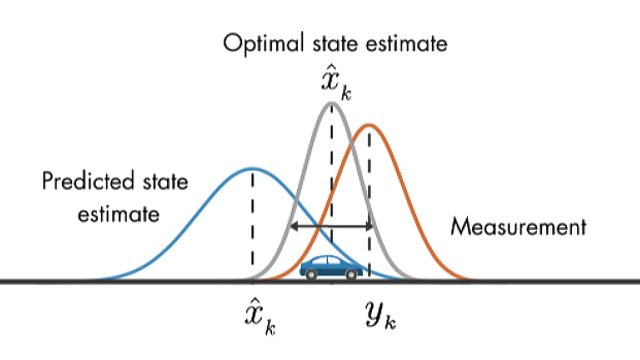
\includegraphics[width=1.0\linewidth]{Pictures/State_Estimation/Kalman_Filter/State_Estimate_Illustrated.jpg}
    \caption{Kalman filter estimation principle combining prediction and measurement distributions to produce the optimal state estimate $\hat{\mathbf{x}}_k$. Image taken from MATLAB video on Kalman Filter.\textsuperscript{\cite{kalman_filter}}}
    \label{fig:state-estimation-kalman-filter}
\end{figure}
